% -----------------------------------------------
% Template for JIM
%     jim.sty -> style file
% By Eloi Batlle (eloi@iua.upf.es), changes for 
% ICMC by Bram de Jong (bdejong@iua.upf.es)
% changes for JIM 2007 by Dominique Fober (fober@grame.fr)
% changes for JIM 2009 by Olivier Tache (olivier.tache@imag.fr)
% -----------------------------------------------

\documentclass{article}
\usepackage{jim,amsmath}
\usepackage[utf8]{inputenc}
\usepackage[francais]{babel}
\usepackage[T1]{fontenc}
%\usepackage{pxfonts}
\usepackage{graphicx}
\usepackage{url}
\usepackage{verbatim}


% Title.
% ------
\title{Composition de partitions musicales}

% Single \textsc{address}
% To use with only one author or several with the same address
% ---------------
\oneauthor
 {D. Fober, Y. Orlarey, S. Letz} {
 Grame - Centre national de création musicale \\ 
\{fober, orlarey, letz\}@grame.fr
 }

% Two addresses
% --------------
%\twoauthors
%  {First author} {School \\ Department}
%  {Second author} {Company \\ Address}

% Three addresses
% --------------
%\threeauthors
%  {Auteur 1} {Organisme \\ Adresse électronique}
%  {Auteur 2} {Organisme \\ Adresse électronique}
%  {Auteur 3} {Organisme \\ Adresse électronique}



%____________________________________________________________
\sloppy
\newenvironment{contentsmall}	{\small}

\newenvironment{gmncode}		{\vspace{-2mm}\small\verbatim}{\endverbatim\vspace{-2mm}}


\newcommand{\GMN}			{\emph{Guido Music Notation}}
\newcommand{\Guido}		{\textsc{Guido}}
\newcommand{\GAR}			{GuidoAR}
\newcommand{\syntax}[1]	{\vspace{-3mm} \small #1}
\newcommand{\code}[1]		{{\small \texttt{#1}}}
\newcommand{\gtag}[1]		{$\backslash$\code{#1}}
\newcommand{\oend}			{\emph{fin-ouverte}}
\newcommand{\obeg}			{\emph{début-ouvert}}
\newcommand{\codeindent}	{\\ \hspace*{9mm}}
\newcommand{\rulenum}[1]	{\textbf{#1}}


\begin{document}
%
\maketitle
%
\begin{abstract}
Basé sur le format de notation musicale \Guido , nous avons développé un ensemble d'outils pour la composition de partitions musicales. Il s'agit d'opérations de transformation de haut niveau, prenant des partitions en entrée pour en générer de nouvelles  en sortie. Ces opérations peuvent par exemple s'appliquer au domaine temporel (e.g. couper le début ou la fin d'une partition) ou concerner la structure de la partition (mise en séquence, en parallèle).
La définition d'opérateurs applicables au niveau de la notation permet d'englober l'expression d'idées musicales et leur composition dans une même métaphore. Cela soulève toutefois un certain nombres de problèmes liés à la cohérence de la notation.
Cet article donne un aperçu du format de notation musicale \Guido , puis il présente les opérations de composition de partitions, les problèmes qui se posent pour la cohérence de la notation et les solutions proposées.
\end{abstract}

%----------------------------------------------------------------
\section{Introduction}\label{sec:intro}
%----------------------------------------------------------------
Le format de notation musicale \Guido\ [GMN] \cite{hoos98} \cite{guido} a été définit par H. Hoos et K. Hamel il y a plus de 10 ans.
Il est très proche du format adopté par Lilypond \cite{lilypond03} \cite{lilypond06} mais il est apparu antérieurement.
Le format GMN est un langage textuel de représentation de partitions musicales. Il est basé sur un formalisme simple mais puissant, se concentrant sur les grands concepts musicaux (en opposition aux caractéristiques graphiques). L'approche développée par \Guido\ repose sur l'idée \emph{d'adéquation}, qui invite à noter simplement les concepts musicaux simples, et à ne recourir à des notations complexes que pour les notions musicales complexes.

Basée sur le format GMN, la librairie \Guido\ \cite{daudin09a,Fober:04b} fournit un puissant moteur de mise en page de partitions, qui se différencie notamment des approches de type \emph{compilateur}  \cite{lilypond03,musixtex} par sa capacité à être embarquée dans une application indépendante, et par la rapidité et l'efficacité du moteur de rendu, qui le rendent utilisable dans un contexte \emph{temps réel} pour des partitions simples.

Basées sur la combinaison du langage et du moteur de rendu \Guido , des opérations de composition de partitions ont été développées : opérations de transformation rythmique, de hauteur, de sélection temporelle ou événementielle, de mise en séquence ou en parallèle, etc.

La notation musicale reste l'une des représentations les plus utilisées par les musiciens. La définition d'opérateurs de composition de partitions constitue un moyen homogène de concilier écriture et transformation tout en restant à un haut niveau de description symbolique de la musique. De plus, la conception de ces opérateurs permet d'utiliser des partitions tant comme cible que comme argument de ces opérations, renforçant la métaphore de la notation comme support d'idées musicales aussi bien que d'opérations de composition.

Toutefois, ces opérations de composition de partitions musicales soulèvent un certain nombre de problèmes liés à la cohérence de la notation. Comme élément de réponse à ces problèmes, nous proposons une typologie simple des éléments de notation musicale ainsi qu'un ensemble de règles de composition basées sur cette typologie.

Cet article donnera quelques rappels sur le format de notation \Guido , les sections suivantes présenteront les opérations de composition de partitions, les problèmes soulevés par ces opérations et les solutions proposées. Nous proposerons ensuite une extension du langage GMN pour prendre  en compte la réversibilité des opérations.

%----------------------------------------------------------------
\section{Le format de notation Guido}
%----------------------------------------------------------------

\subsection{Concepts de base}
%----------------------------------------------------------------
Le format de base de \Guido\ recouvre les notes, silences, altérations, voix indépendantes, et les concepts les plus courants de la notation musicale comme les clefs, métriques, armures, articulations, liaisons, etc.
Les notes sont représentées par leur nom \texttt{(a b c d e f g h)}, une altération optionnelle ('\#' et '\&' pour dièse et bémol), un numéro d'octave optionnel et une durée optionnelle. \\
La durée est spécifiée par l'une des formes suivantes: 
\begin{gmncode} 
   '*'enum'/'denom dotting
   '*'enum dotting 
   '/'denom dotting
\end{gmncode} 
\noindent où $enum$ et $denom$ sont des entiers positifs et $dotting$ est soit vide, '.', ou '..', avec la même sémantique que dans la notation musicale. 1 est la valeur par défaut si $enum$ ou $denom$ sont omis. La durée exprime une fraction de ronde.

Si omises, les valeurs optionnelles sont les dernières utilisée pour la note précédente de la séquence.

Les accords sont décrits par des notes entre accolades séparées par des virgules, i.e. \code\{{c, e, g}\}


\subsection{Tags \Guido}
%----------------------------------------------------------------
Les tags sont utilisés pour donner des informations musicales supplémentaires, comme les liaisons, clés, armures, etc. Un tag a l'une des formes suivantes:
\begin{gmncode} 
   \tagname 
   \tagname<param-list>
\end{gmncode}
\noindent où \code{param-list} est une liste de chaînes de caractères ou de nombres, séparés par des virgules. Un tag peut avoir une étendue temporelle et s'appliquer à un ensemble de notes (par ex. les liaisons) ; la forme correspondante est:
\begin{gmncode} 
   \tagname(note-series)
   \tagname<param-list>(note-series)
\end{gmncode} 

Le code GMN suivant illustre la concision de la notation ; la figure \ref{ex1} donne le rendu effectué par le moteur \Guido. 
\begin{gmncode} 
  [ \meter<"4/4"> \key<-2> c d e& f/8 g ]
\end{gmncode} 

\begin{figure}[h]
	\centering 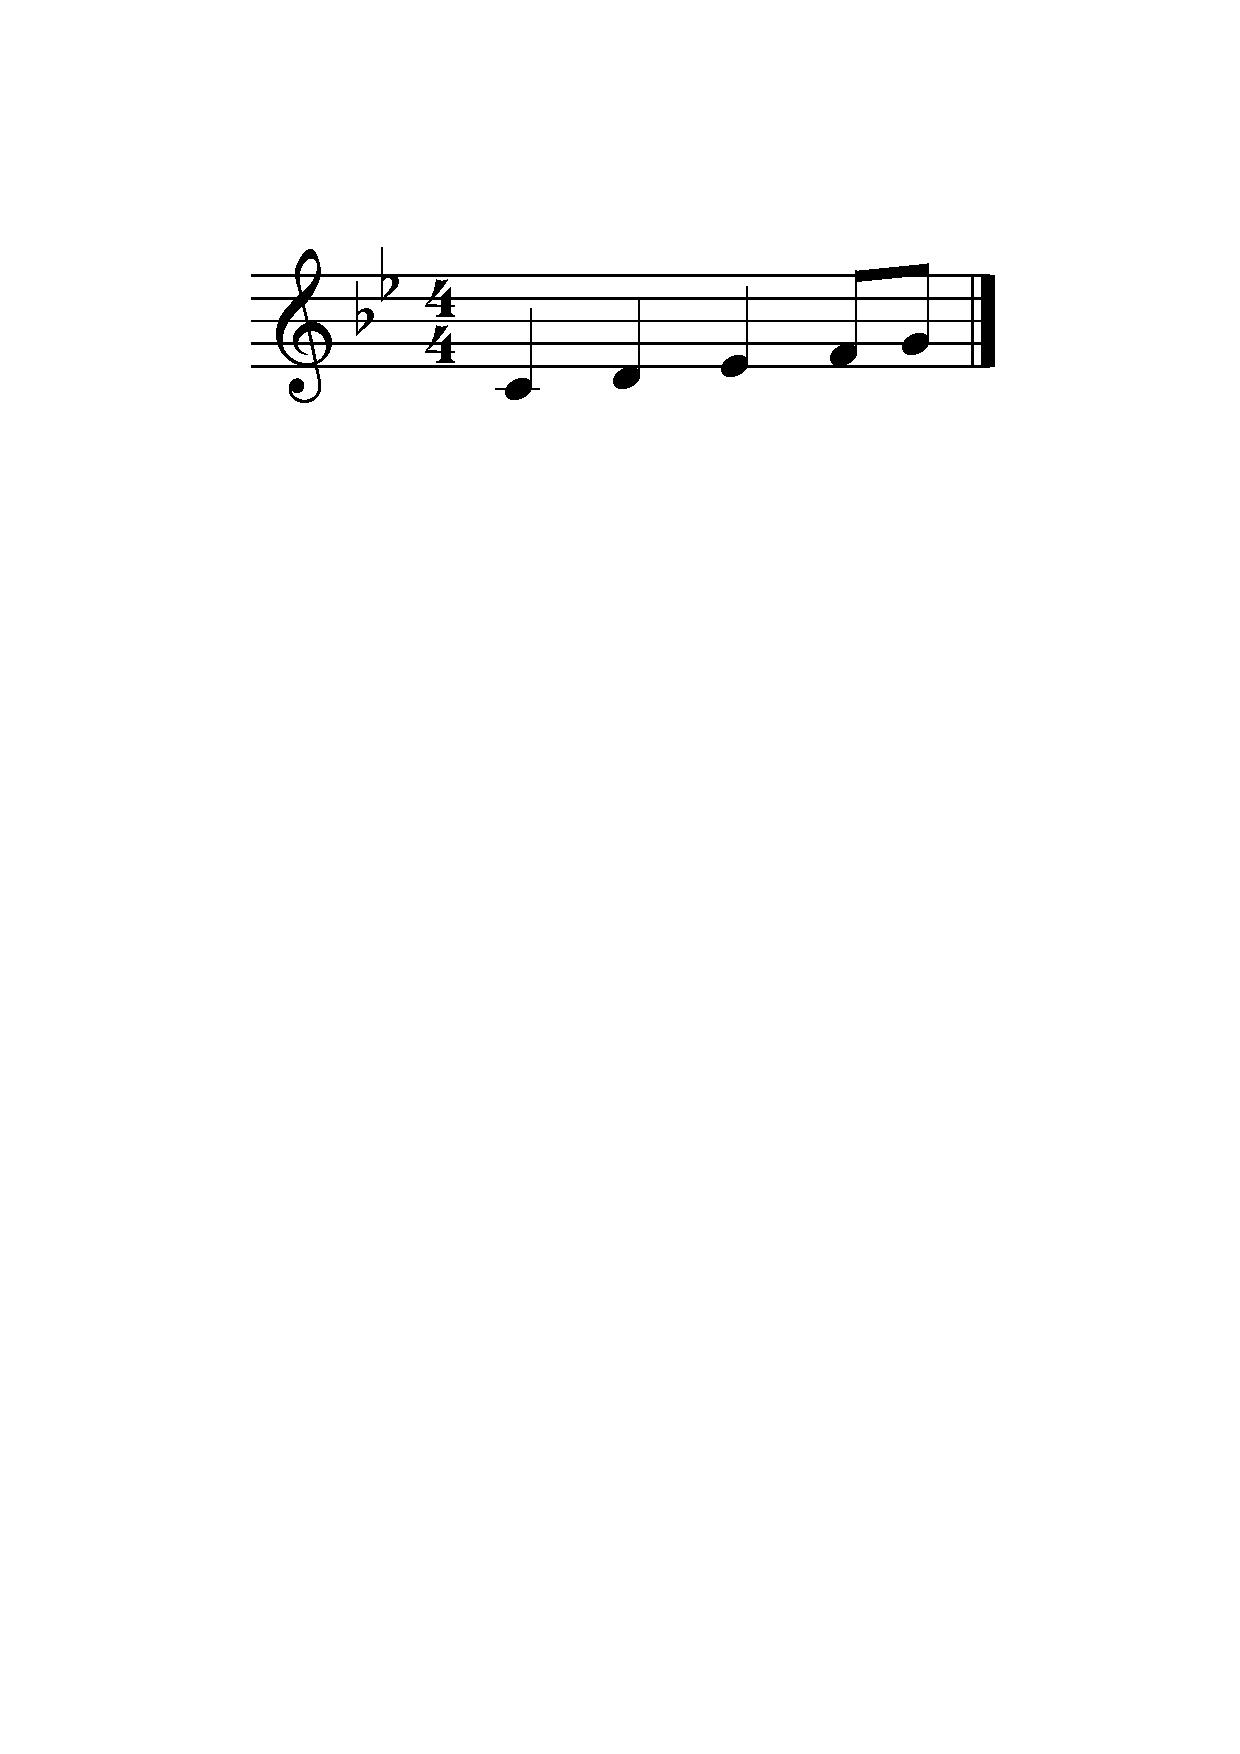
\includegraphics[width=47mm]{imgs/ex1}
 \caption{Un exemple GMN simple}
 \label{ex1}
\end{figure}


\subsection{Séquences et segments}
%----------------------------------------------------------------
Une séquence de notes a la forme \verb+[tagged-notes]+ où \code{tagged-notes} est une série de notes, tags, tags temporels séparés par des espaces. Une séquence de notes représente une seule voix.
Les segments de notes représentent plusieurs voix ; ils sont notés par \verb+{seq-list}+ où \code{seq-list} est une liste de séquences de notes séparées par des virgules, comme dans l'exemple suivant (figure \ref{fig:voices}):
\codeindent\code{ \{ [ e g f ], [ a e a ] \} }
\begin{figure}[h]
	\centering 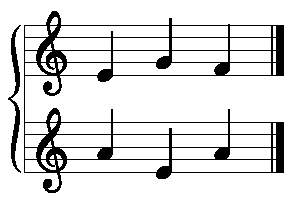
\includegraphics[width=32mm]{rsrc/voices}
 \caption{Exemple à plusieurs voix}
 \label{fig:voices}
\end{figure}


\subsection{\Guido\ Avancé}
%----------------------------------------------------------------
Le format \Guido\ Avancé inclus des tags supplémentaires et un contrôle plus fin de la mise en page.
Il définit notamment des paramètres tels que $dx$ et $dy$ pour ajuster le positionnement des éléments de la partition. Il autorise le formatage de notes et de silences, les assignations à des portées, etc.
Un exemple de code est donné ci-dessous avec le rendu correspondant (figure \ref{advex}).

\begin{gmncode} 
{
 [
  \barFormat<"system">
  \staff<1> \stemsUp \meter<"2/4"> 
  \intens<"p", dx=1hs,dy=-7hs>
  \beam(g2/32 e/16 c*3/32) c/8 
  \beam(\noteFormat<dx=-0.9hs>(a1/16) c2 f) 
  \beam(g/32 d/16 h1*3/32) d2/8 
  \beam(h1/16 d2 g)],
 [\staff<1>\stemsDown g1/8 e
  f/16 \noteFormat<dx=0.8hs>(g) f a a/8 e 
  f/16 g f e],
 [\staff<2> \meter<"2/4"> 
  \stemsUp a0 f h c1],
 [\staff<2> \stemsDown c0 d g {d, a}]
}
\end{gmncode} 

\begin{figure}[h]
	\centering 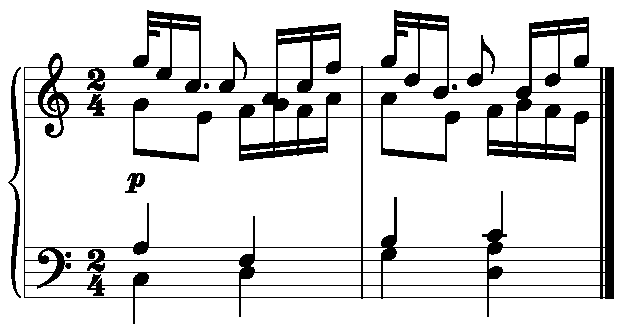
\includegraphics[width=0.85\columnwidth]{rsrc/4voices}
 \caption{Exemple \Guido\ Avancé}
 \label{advex}
\end{figure}



%----------------------------------------------------------------
\section{Composition de partitions}
%----------------------------------------------------------------
\subsection{Operations}
Des opérations de composition de partitions ont été implémentées sous forme de librairie indépendante (\GAR ). Elles sont décrites par la table  \ref{operations}. Ces opérations sont disponibles sous forme d'API, d'utilitaires pour la ligne de commande, ou encore dans l'environnement graphique d'une application indépendants : \Guido Calculus.
La plupart de ces opérations prennent une partition et une valeur en entrée pour produire une nouvelle partition en sortie. La valeur passée en entrée peut-être donnée sous forme de partition: par exemple, l'opération  \code{top} coupe les voix d'une partition après un nombre de voix $n$ ; en utilisant une partition à la place de ce paramètre, c'est le nombre de voix de cette partition qui sera pris comme valeur.
Ainsi, toutes les opérations peuvent se décrire de manière homogène au niveau symbolique de la notation. 

Ce design permet également d'exprimer des séries de transformations en ligne de commande, comme le pipe-line de partitions à travers de opérateurs e.g. \\
\hspace*{4mm} \code{head s1 s2 | par s2 | transpose "[ c ]" }

\begin{table*}[htdp]
\begin{center}
\begin{tabular}{rcl}
\hline
operation & args		&	description \\
\hline
seq 	&	$s1\ s2$		& met $s1$ et $s2$ en séquence \\
par 	&	$s1\ s2$		& met $s1$ et $s2$ en parallèle \\ 
rpar	&	$s1\ s2$		& met $s1$ et $s2$ en parallèle, alignés à droite \\
top 	&	$s1\ [n\ | \ s2]$ 	& prend les $n$ premières voix de $s1$; \\
		&	& quand  on utilise une partition $s2$ comme paramètre, $n$ est le nombre de voix de $s2$ \\
bottom 	&	$s1\ [n\ | \ s2]$ 	& coupe les $n$ première voix de $s1$;  \\
		&	& quand  on utilise une partition $s2$ comme paramètre, $n$ est le nombre de voix de $s2$ \\
head	& 	$s1\ [d\ | \ s2]$	& prend le début de $s1$ jusqu'à la date $d$; \\
		& 	& quand  on utilise une partition $s2$ comme paramètre, $d$ est la durée de $s2$ \\
evhead 	&	$s1\ [n\ | \ s2]$	& prend les $n$ premiers événements $s1$ ; \\
		& 	& quand  on utilise une partition $s2$ comme paramètre, $n$ est le nombre d'événements de $s2$ \\
tail	&	$s1\ [d\ | \ s2]$ 	& coupe le début de $s1$ jusqu'à la date $d$; \\
		& 	& quand  on utilise une partition $s2$ comme paramètre, $d$ est la durée de $s2$ \\
evtail 	&	$s1\ [n\ | \ s2]$ 	& coupe les $n$ premiers événements de $s1$ ; \\
		& 	& quand  on utilise une partition $s2$ comme paramètre, $n$ est le nombre d'événements de $s2$ \\
transpose 	&	$s1\ [i\ | \ s2]$	& transpose $s1$ d'un intervale $i$; \\
			& 	& quand  on utilise une partition $s2$ comme paramètre, $i$ est calculé comme la différence  \\
			& 	& entre la première note de la première voix de $s1$ et $s2$ \\
duration 	&	$s1\ [d\ |\ r\ |\ s2]$	& étire $s1$ à une durée $d$ ou selon un facteur $r$; \\
			& 	& quand  on utilise une partition $s2$ comme paramètre, $d$ est la durée de $s2$ \\
applypitch 	&	$s1\ s2$	& applique les hauteurs de $s1$ à $s2$ en boucle \\
applyrythm 	&	$s1\ s2$	& applique le rythme de $s1$ à $s2$ en boucle \\
\hline
\end{tabular}
\end{center}
\caption{Opérations sur les partitions}
\label{operations}
\end{table*}

%----------------------------------------------------------------
\subsection{Les problèmes de notation}
\label{issues}
Dans les faits, les fonctions de composition de partition opèrent sur une représentation en mémoire de la notation musicale. Toutefois, nous allons illustrer les problèmes liés avec la représentation textuelle qui est équivalente à la représentation mémoire.

Prenons l'exemple de l'opération \code{tail} appliquée à la partition suivante:
\codeindent \code{[\gtag{clef}<"f"> c d e c]}\\
Une coupure \emph{brute} de la partition après 2 notes donne le code \code{[e\ c]} où l'information de clef a disparu, pouvant conduire à un rendu non souhaité (figure \ref{fig:tail}).
\begin{figure}[h]
	\centering 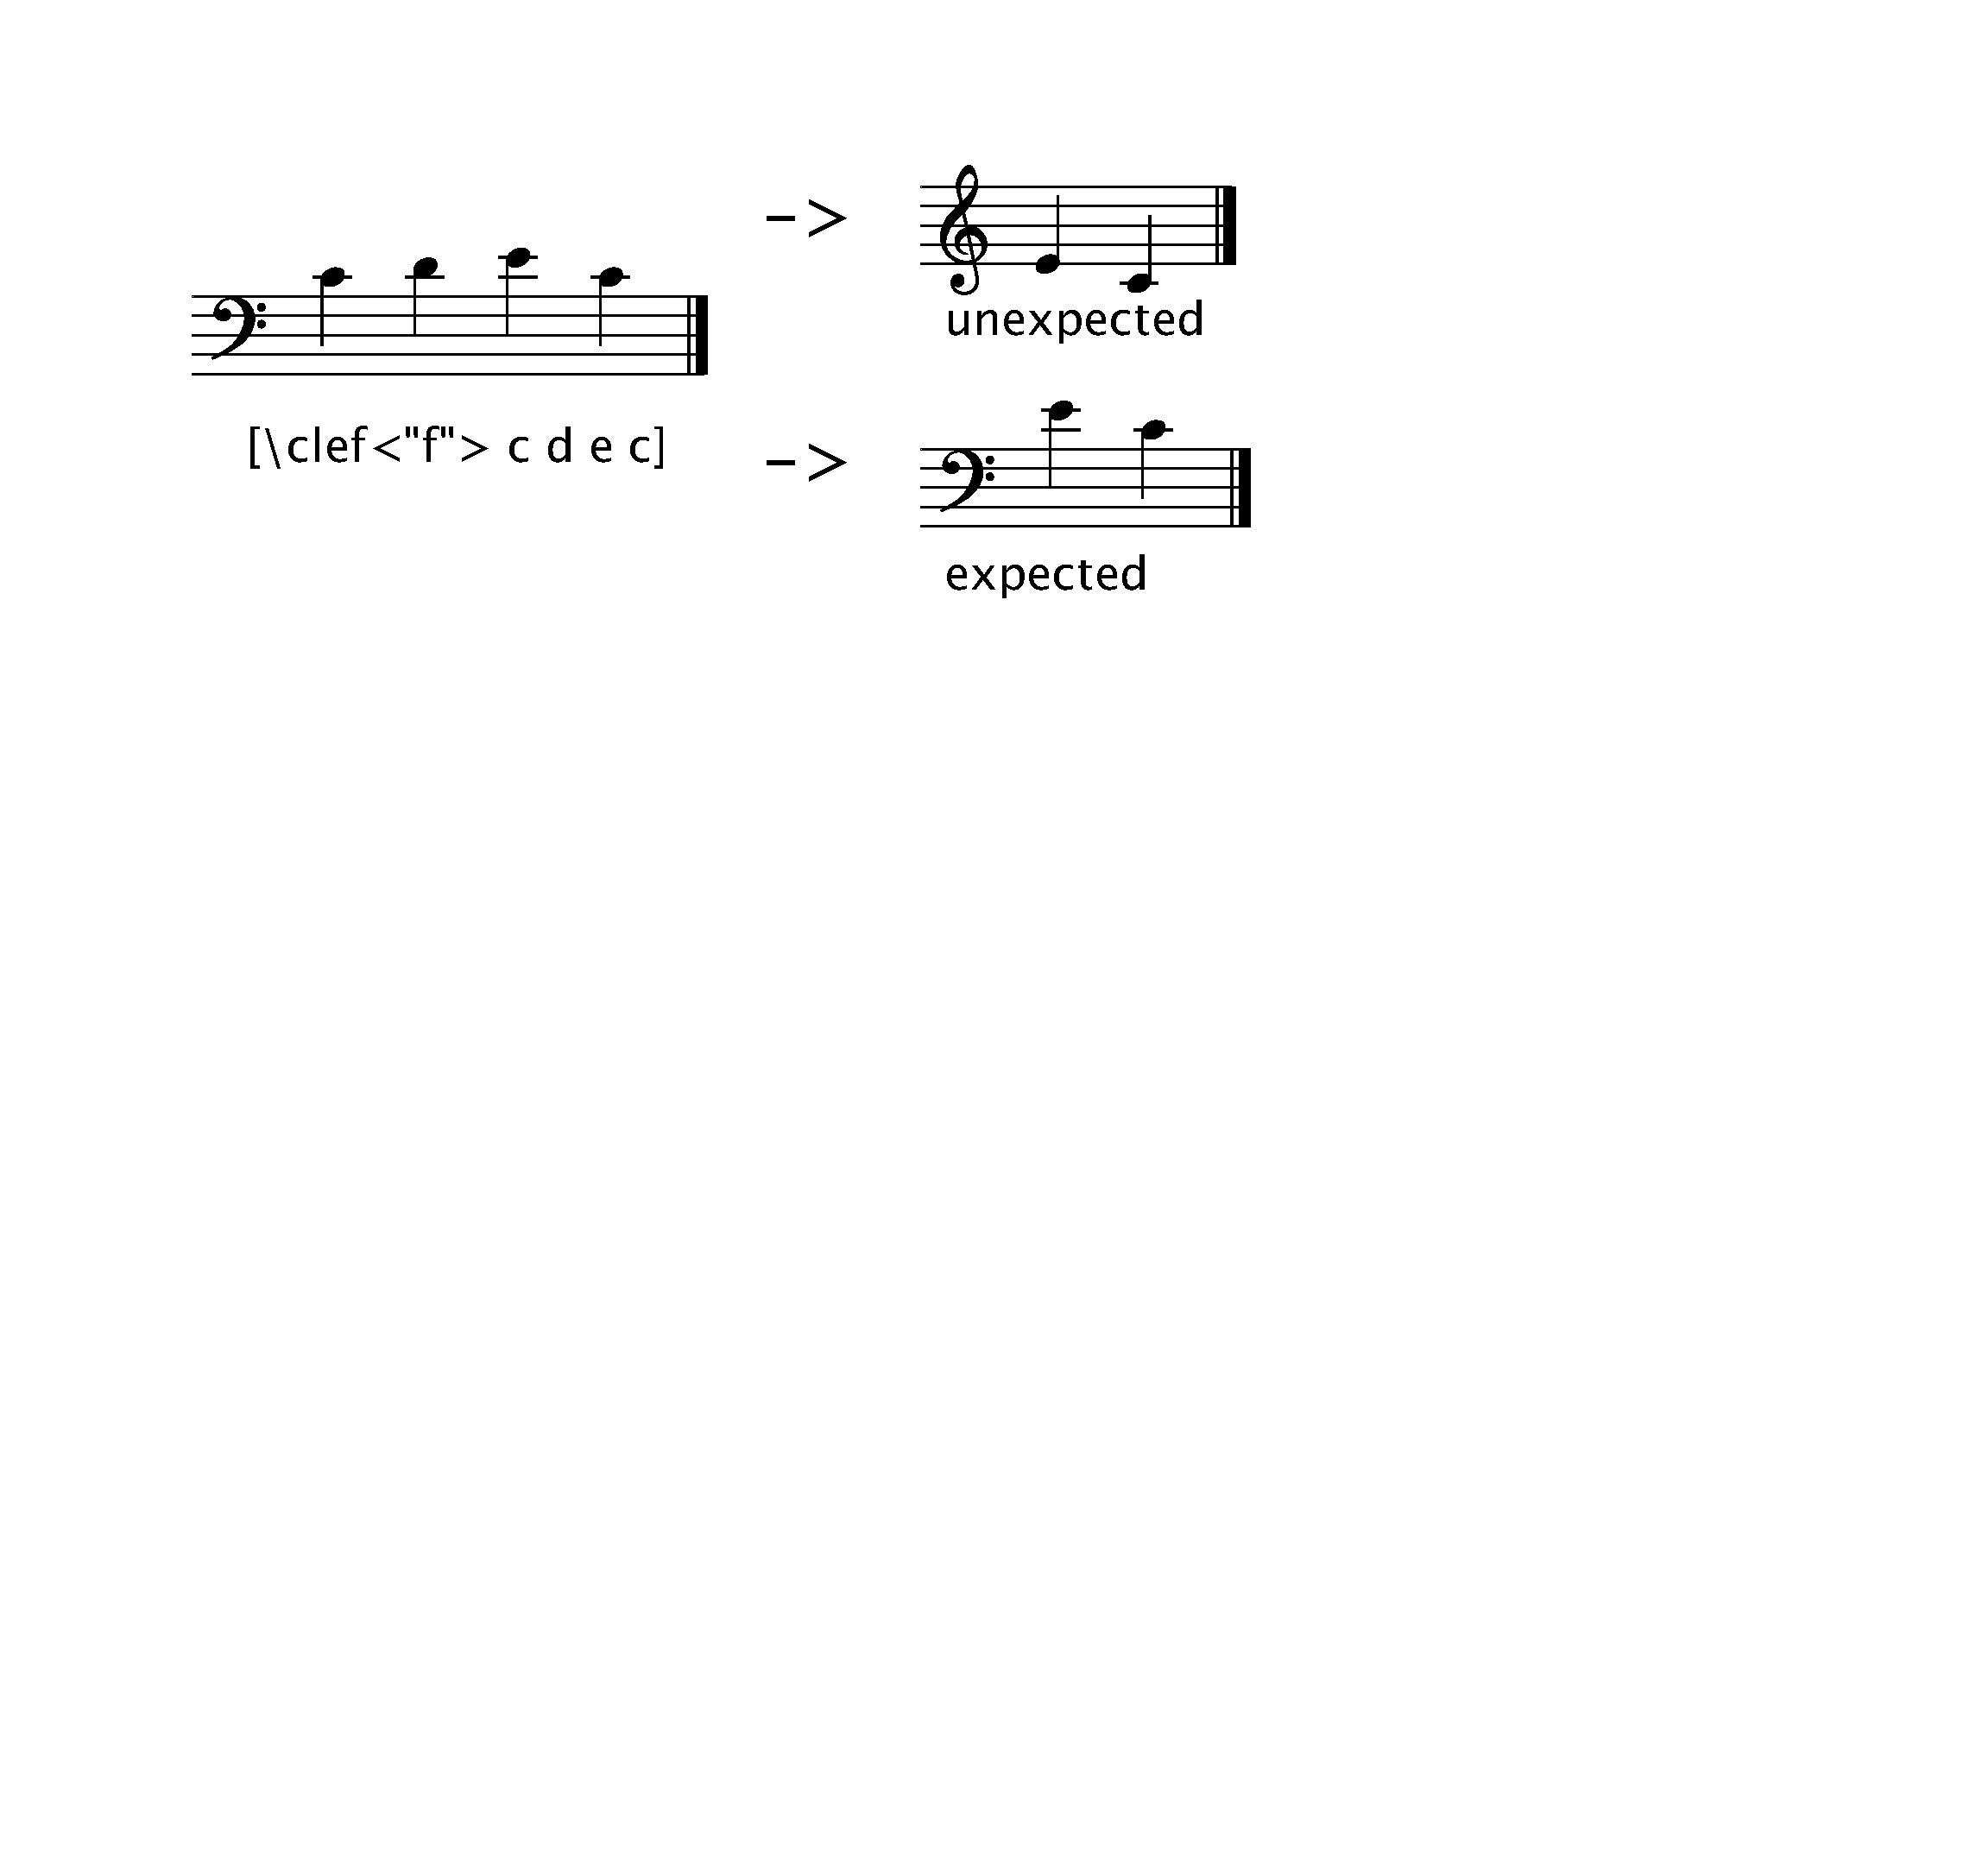
\includegraphics[width=60mm]{imgs/tail}
 \caption{Cohérence de l'opération \code{tail}}
 \label{fig:tail}
\end{figure}

Voici un autre exemple avec l'opération \code{seq} : la mise en séquence de
	\hspace{1mm} \code{[\gtag{clef}<"g"> c d]} \\
et 	\hspace{20.5mm}\code{[\gtag{clef}<"g"> e c]} \\
donnera 	\hspace{7.1mm} \code{[\gtag{clef}<"g"> c d \gtag{clef}<"g"> e c ]} 
où la clef est répétée inutilement (figure \ref{fig:seq2})  ce qui rend la lecture plus confuse.
\begin{figure}[h]
	\centering 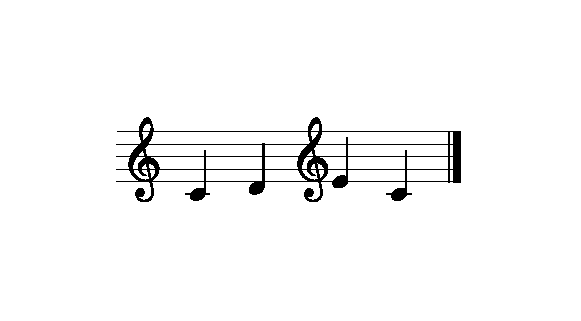
\includegraphics[width=40mm]{imgs/seq2}
 \caption{Mise en séquence \emph{brute}}
 \label{fig:seq2}
\end{figure}

Certaines opérations peuvent également donner des résultats syntactiquement incorrects. Considérons le code suivant :
\codeindent \code{[g \gtag{slur}(f e) c]} \\
le partage de la partition en 2 après \code{f} donnerai 
\codeindent \textbf{a)}\ \ \code{[g \gtag{slur}(f]} \ \  et\ \ \textbf{b)} \ \  \code{[e) c]} \\
i.e. comprenant des tags temporels inachevés. Nous utiliserons les termes tags à \oend\ pour faire référence au cas a) et tag à \obeg\ pour le cas b).

Ces quelques exemples illustrent une partie du problème et il y a beaucoup d'autres cas où la cohérence de la notation doit être préservée lors d'opérations sur les partitions.

%----------------------------------------------------------------
\subsection{Etendue temporelle des éléments}
Nous proposons de traiter le problème en définissant une typologie des éléments de notation en fonction de leur étendue temporelle, et en spécifiant des règles de cohérence basées sur ces types.

Le format GMN fait une distinction entre les tags de position (comme \gtag{clef} ou \gtag{meter}) et les tags temporels (\gtag{slur}, \gtag{beam}, etc.) : 
\begin{itemize}
\item les tags temporels ont une durée explicite : la durée des notes qu'ils contiennent, 
\item les tags de position sont de simples marques de notations à une position donnée. 
\end{itemize}
Cette distinction n'est toutefois pas suffisante pour couvrir le problème : beaucoup de tags de position ont une durée implicite, qui s'étend généralement jusqu'à un signe de de notation similaire ou jusqu'à la fin de la partition. C'est le cas par exemple de la notation de l'intensité.
\begin{table*}[htdp]
\begin{center}
\begin{tabular}{cll}
étendue temporelle & description & exemple \\
\hline
explicite 	& la durée est explicite dans la notation	& slur, cresc \\
implicite 	& la durée s'étend jusqu'au prochain signe similaire ou jusqu'à la fin	& meter, dynamics, key \\
autres 		& contrôle de la structure			& coda, da capo, repeats\\
	- 		& instructions	 de formatage 	& new line, new page \\
	- 		& notations diverses & breath mark, bar \\
\hline
\end{tabular}
\end{center}
\caption{Typologie des éléments de notation.}
\label{types}
\end{table*}

La table  \ref{types} présente une typologie simple des éléments de notation musicale, principalement fondée sur leur étendue temporelle. Nous définissons également la notion \emph{de tag courant} : pour un type de tag d'étendue temporelle implicite donné (clef, meter...), il s'agit de la dernière valeur rencontrée. 

Basées sur cette typologie, des précautions sont à prendre lors des opérations suivantes :

\begin{itemize}
\item calcul du début d'une partition :  
\begin{description}
	\item[1)] tous les tags d'étendue temporelle explicite doivent être ouverts (i.e. les tags à \obeg , voir section \ref{issues})
	\item[2)] les tags courants d'étendue temporelle implicite  doivent être rappelés,
\end{description}
\item calcul de la fin d'une partition : 
\begin{description}
	\item[3)] les tags d'étendue temporelle explicite doivent être fermés (i.e. les tags à \oend )
\end{description}
\item mise en séquence de partitions : 
\begin{description}
	\item[4)] les tags d'étendue temporelle implicite de la deuxième partition doivent être supprimés quand ils correspondent à un tag courant.
\end{description}
\end{itemize}


%----------------------------------------------------------------
\subsection{Structure control issues} \label{sc}
Les éléments qui relèvent de la catégorie \emph{autres / contrôle de la structure} peuvent également donner lieu à des incohérences de notation : une barre de début de répétition sans barre de fin de répétition, un \emph{dal segno} sans \emph{segno}, un \emph{da capo al fine} sans \emph{fine}, etc.
Nous introduisons de nouvelles règles pour la consistance des barres de répétitions. Nous définissons tout d'abord une barre de répétition \emph{en suspens} comme le cas d'une barre de début de répétition sans barre de fin correspondante. 
\begin{itemize}
\item[\rulenum{5)}] lors du calcul de la fin d'une partition, les barres de répétition \emph{en suspens} doivent être fermées avec une barre de fin de répétition.
\item[\rulenum{6)}] dans le cas de barres de début de répétition successives, seule la première sera retenue
\item[\rulenum{7)}] dans le cas de barres de fin de répétition successives, seule la dernière sera retenue
\end{itemize}

Il n'y a pas de préconisation particulière pour les autres éléments de contrôle de la structure : les incohérences qui peuvent se produire sont ignorées mais ce choix préserve la réversibilité des opérations.


%----------------------------------------------------------------
\subsection{Réversibilité des opérations}\label{reverse}
Les règles définies ci-dessus résolvent la majorité des problèmes de notation mais ne permettent pas d'inverser les opérations : considérons une partition comportant une liaison qui est coupée en son milieu et rassemblée par une mise en séquences. Le résultat comportera deux liaisons (figure \ref{fig:rev}) en raison des règles \rulenum{1)} et \rulenum{3)} qui forcent l'ouverture des tags à \obeg\ et la fermeture des tags à \oend .
\begin{figure}[h]
	\centering 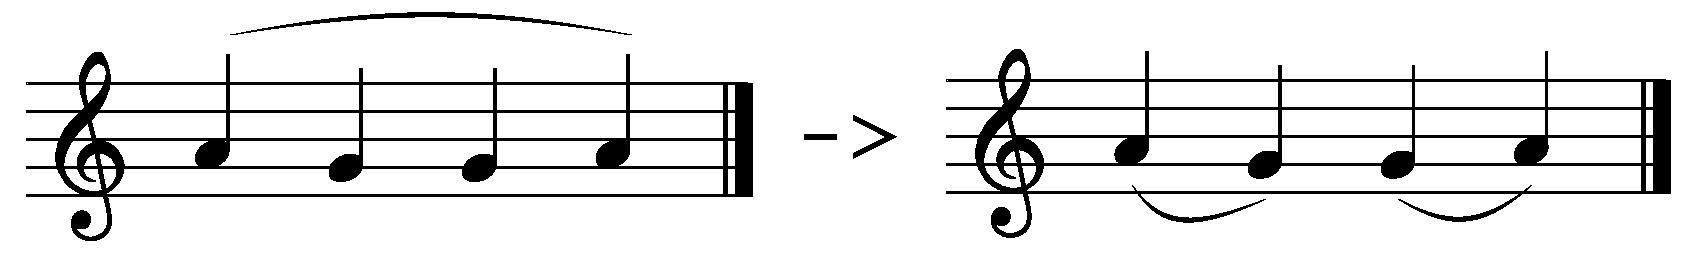
\includegraphics[width=80mm]{imgs/reverse}
 \caption{Une partition découpée et remise en séquence}
 \label{fig:rev}
\end{figure}

La résolution du problème requiert le support du langage GMN : nous introduisons un nouveau paramètre pour les tags d'étendue temporelle explicite, conservant l'histoire du tag et indiquant un antécédent de type \oend\ et/ou \obeg\ .
Ce paramètre est de la forme : 
\codeindent \code{\gtag{tag}<open="type">} \\
où \code{type} est parmi [\code{begin}, \code{end}], correspondant respectivement à des antécédents \obeg\ et \oend .

Nous introduisons ensuite une nouvelle règle pour la composition de partitions, qui nécessite de définir des \emph{tags adjacents} comme des tags placés sur la même voix et qui ne sont séparés par aucune note ou accord.
\begin{itemize}
\item[\rulenum{8)}] les tags \emph{adjacents} similaires qui portent un paramètre \code{open} s'annulent mutuellement quand le premier est de type \oend\ et le second \obeg .
\end{itemize}
Ainsi, une opération rencontrant une forme de type :
\codeindent \code{\gtag{anytag}<open="end">(f g) 
\codeindent \gtag{anytag}<open="begin">(f e)} \\
la transformera en :
\codeindent\code{\gtag{anytag}(f g f e)} 


%----------------------------------------------------------------
\section{Conclusion}
%----------------------------------------------------------------

La complexité de la notation musicale repose en grande partie sur le grand nombre d'éléments de notation et sur leur statut hétérogène. La typologie que nous avons proposé (table \ref{types}) en est une simplification arbitraire, destinée à couvrir les besoins d'opérations de composition de partitions. Elle n'est  pas représentative de cette complexité mais comme elle se base sur la sémantique de la notation, elle peut être appliquée à tout format de représentation de la notation musicale.
Hormis les règles de réversibilité définies en \ref{reverse} qui nécessitent le support du langage de représentation de la musique pour opérer, toutes les autres règles sont indépendantes du format GMN.

Les opérations sur les partitions peuvent se révéler très utiles dans le cas de traitements par lot (par exemple : séparation des voix d'un conducteur, extraction d'extraits, etc.).  Les opérateurs présentés en table \ref{operations} permettent ce type de traitement, mais ouvrent également la voie à de nouvelles approches créatives de la musique.

\bibliographystyle{unsrt}
\bibliography{../guido}

\end{document}
